\chapter{EquiDiff: Equivariant Diffusion Sampling for Invariant Set Generation}\label{r:method}

This chapter presents the theoretical foundation and algorithmic details of our proposed approach for generating invariant sets of neural network representations. We begin with formal mathematical definitions, establish the relationship to classical level sets from differential topology \citep{lee2013smooth,milnor1965topology,fort2017gaussian}, detail our core algorithm, and conclude with implementation specifics and quality assurance measures.

\section{Theoretical Foundation and Formal Definitions}

We begin by establishing the mathematical foundations for our approach through formal definitions that clarify the key concepts and their relationships.

\begin{defi}[Invariant Framework]\label{def:invariants_framework}
Let $f: \mathbb{R}^n \rightarrow \mathbb{R}^m$ be a neural network with $n$ input dimensions and $m$ output dimensions, where $n$ represents the dimensionality of the input space (e.g., $n = W \times H \times C$ for images of width $W$, height $H$, and $C$ channels) and $m$ represents the dimensionality of the network component we wish to analyze (e.g., $m = 1$ for a single neuron, $m = k$ for $k$ class logits). The network $f$ can be viewed as a composition of functions $f = f_L \circ f_{L-1} \circ \ldots \circ f_1$, where each $f_i$ represents a layer transformation.

For a given query point $\mathbf{x}^* \in \mathbb{R}^n$, the \textbf{Invariant Framework} defines the theoretical foundation for identifying all inputs that produce identical network responses under a specified objective function.
\end{defi}

\begin{defi}[EquiDiff Method]\label{def:equidiff_method}
Given the Invariant Framework (Definition \ref{def:invariants_framework}), we define the \textbf{EquiDiff method} as an algorithmic approach that combines score-based diffusion models with infinite optimization to generate diverse, realistic samples from invariant sets.

Specifically, for a neural network $f: \mathbb{R}^n \rightarrow \mathbb{R}^m$ and query point $\mathbf{x}^*$, EquiDiff generates samples $\{\mathbf{x}_i\}_{i=1}^N$ through three integrated mechanisms. The method maintains an invariance constraint by ensuring $\|f(\mathbf{x}_i) - f(\mathbf{x}^*)\|_2 < \epsilon$ for small $\epsilon > 0$, where the $L_2$ distance between network outputs remains below a specified threshold. Simultaneously, a realism constraint ensures that generated samples $\mathbf{x}_i$ lie within the natural image manifold as defined by a pre-trained diffusion model, preventing the generation of adversarial artifacts or unrealistic patterns. Finally, a diversity constraint promotes semantic and visual variety among generated samples while preserving the strict invariance requirement, enabling exploration of the full breadth of patterns that activate identical network responses.

The method operates through infinite optimization over the latent space of a diffusion model, enabling precise control over network activations while ensuring realistic image generation through the inherent properties of the diffusion sampling process.
\end{defi}

\begin{figure}[h]
\centering
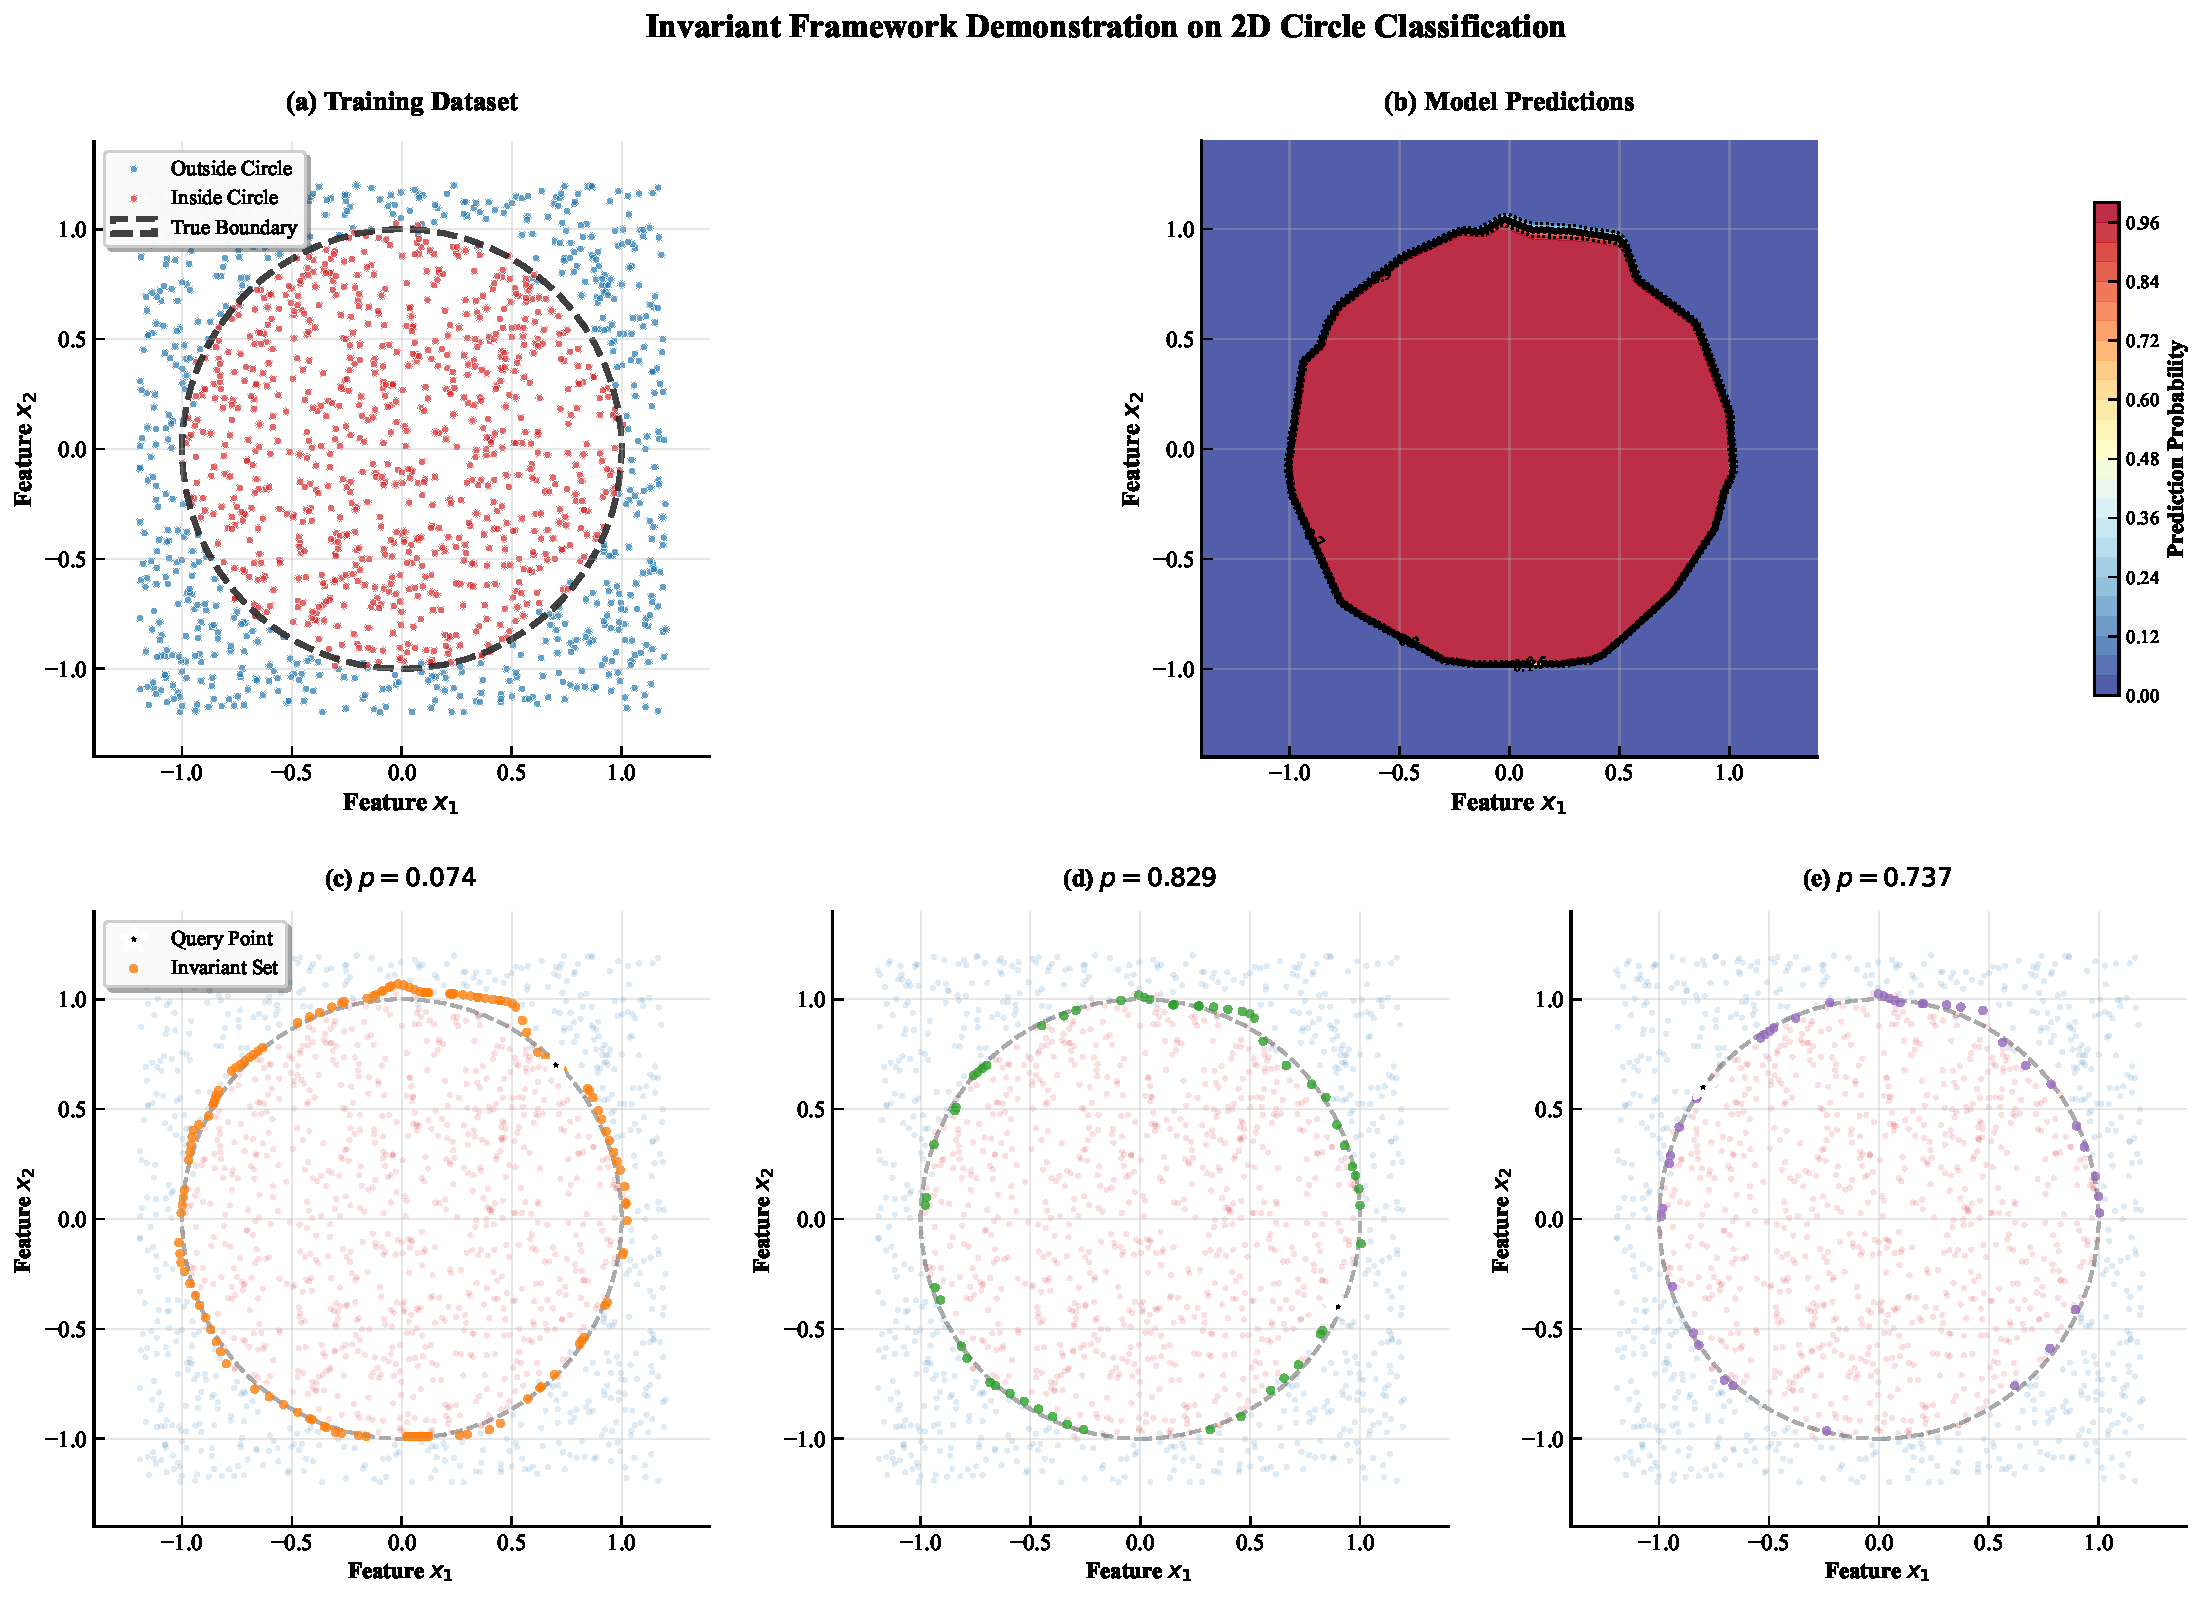
\includegraphics[width=\linewidth]{figures/main/invariant_framework_combined.pdf}
\caption{Demonstration of the Invariant Framework on a 2D Concentric Circles Dataset.
(a) Training dataset with 1,500 samples classified by their position relative to a unit circle (dashed line). Blue points represent the outer class, pink points the inner class.
(b) Learned decision boundary and prediction probability heatmap from a 3-layer MLP (test accuracy: 0.983). The black contour shows the 0.5 decision boundary.
(c-e) Invariant sets for three query points (black stars) with prediction values p. Orange points represent all input locations that yield identical predictions under the trained model, demonstrating the equivalence relation established by the model's output. The invariant sets approximate level curves of the learned decision function, revealing the geometric structure of the model's decision space.}
\label{fig:teaser}
\end{figure}

\begin{figure}[h]
\centering
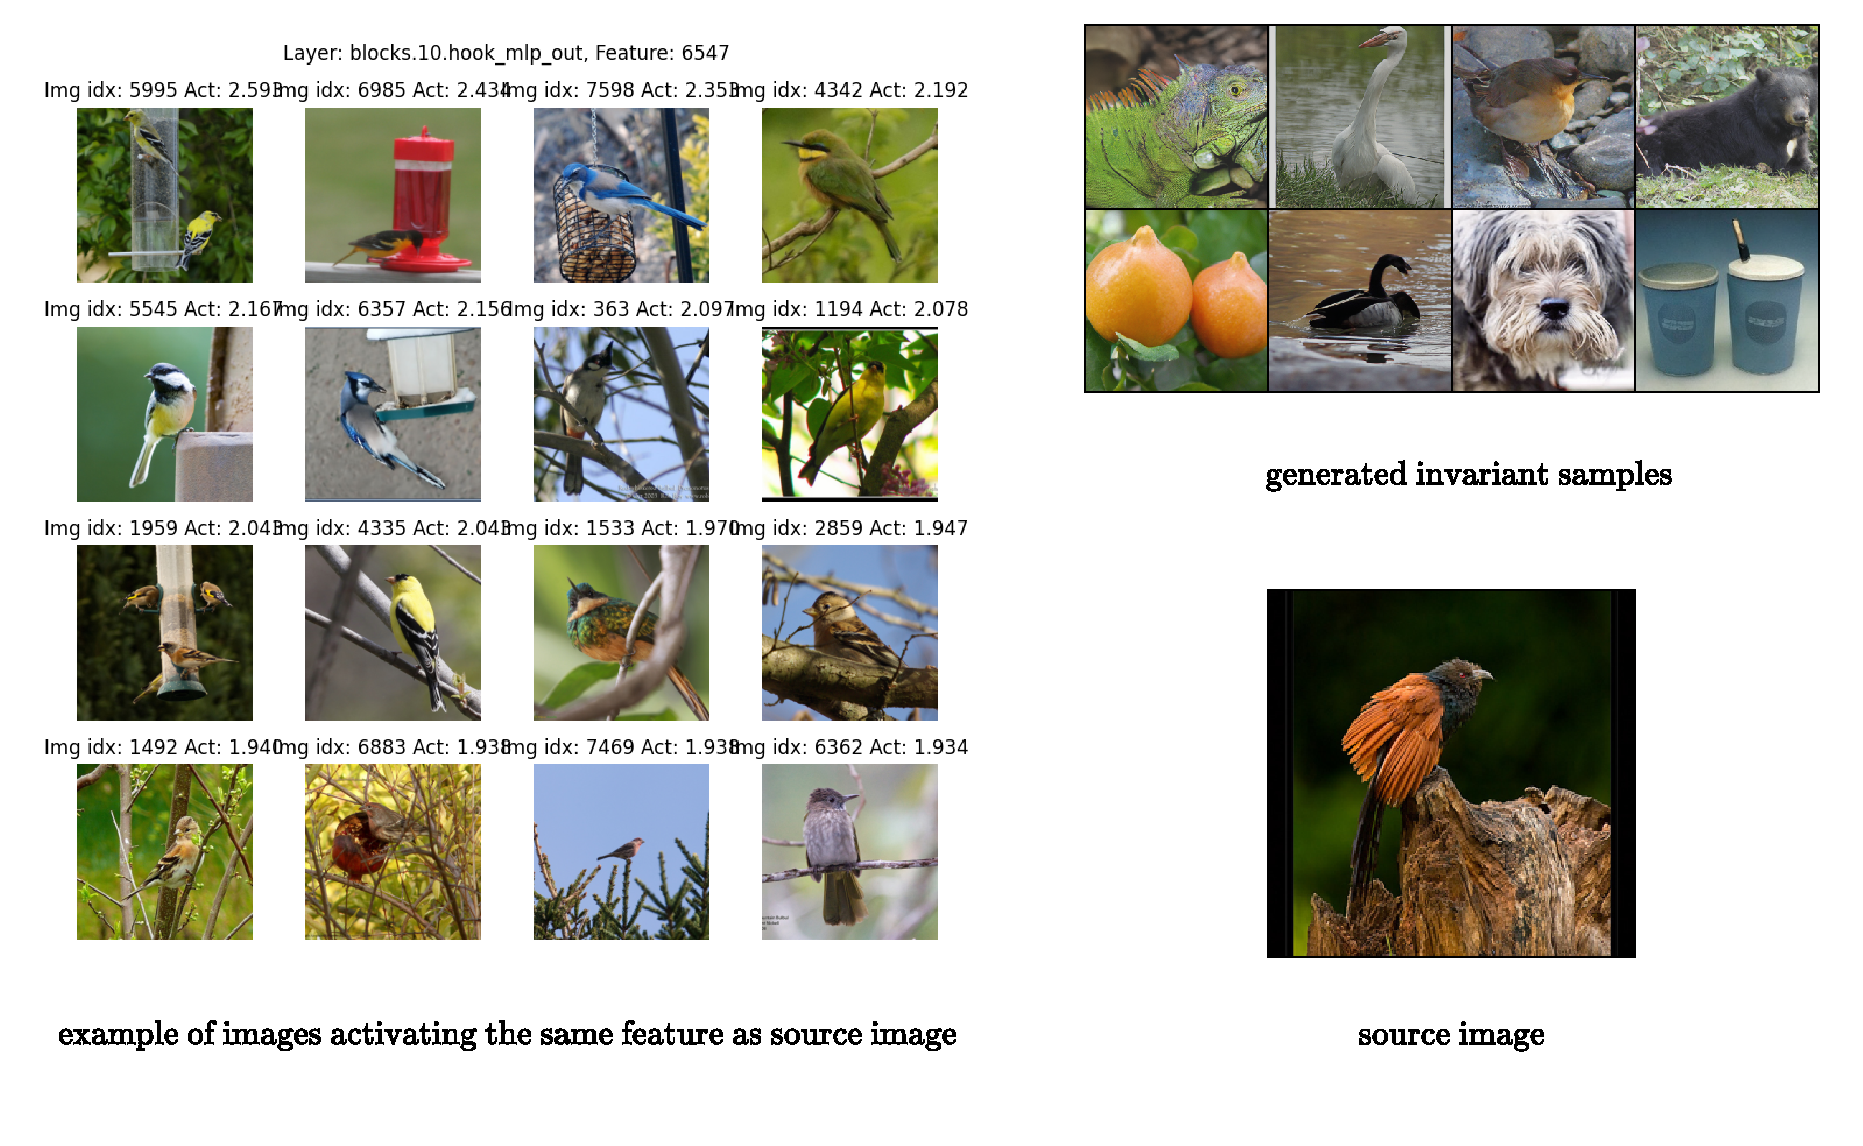
\includegraphics[width=\linewidth]{figures/main/experiment1.2.pdf}
\caption{Real-world demonstration of invariant set generation on sparse autoencoder features from Vision Transformer models. \textbf{Left}: Representative real images from the training dataset that naturally activate SAE feature \#6547, establishing the ground truth semantic concept. \textbf{Top right}: Generated samples from the invariant set using EquiDiff with 512 optimization steps. All generated images achieve tight activation matching with L2 loss $\approx 0.01$ relative to the target activation level, which is ~1.5, demonstrating mathematical precision in invariant set membership. The generated samples reveal the broader visual manifold of patterns that trigger identical feature responses, extending beyond the original training examples to include novel compositions, lighting conditions, and stylistic variations while preserving the core semantic concept. This result validates the Invariant Framework on complex, real-world models rather than toy examples.}
\label{fig:method_sae_demo}
\end{figure}

\section{Problem Formulation}
The problem of finding invariant sets (IS) is formulated as discovering members of an equivalence relation. Given a neural network with parameters $\boldsymbol{\theta}$ and objective function $\mathcal{L}_{\boldsymbol{\theta}}:\mathbb{R}^n \rightarrow \mathbb{R}^m$, and a query point $\mathbf{x^*}$, the invariant set is defined as:
\begin{equation}
  \mathbf{IS}(\mathbf{x^*}) = \{ \mathbf{x} \in \mathbb{R}^n : \mathcal{L}_{\boldsymbol{\theta}}(\mathbf{x}) = \mathcal{L}_{\boldsymbol{\theta}}(\mathbf{x^*}) \}
  \label{eq:is}
\end{equation}
We use the notation $\mathbf{x^*} \sim_{\mathcal{L}_{\boldsymbol{\theta}}} \mathbf{x}$ to denote that two elements $\mathbf{x^*}$ and $\mathbf{x}$ belong to the same invariant set under the equivalence relation defined by $\mathcal{L}_{\boldsymbol{\theta}}$.

The objective function $\mathcal{L}_{\boldsymbol{\theta}}$ can represent various neural network components: a single neuron's activation, class logits for one or multiple classes, or any differentiable function for which gradients can be computed. While adversarial examples can be viewed as specific perturbations that may belong to invariant sets under certain conditions \citep{szegedy2014intriguingpropertiesneuralnetworks}, the goal of this work is fundamentally different: one seeks to sample from the intersection of the invariant set with the natural data manifold, ensuring realism by construction.

To achieve this, this work utilizes a trained diffusion model, specifically LightningDIT \citep{yao2025vavae} \citep{yao2024fasterdit}, which excels at generating high-quality images while maintaining the mathematical constraints of invariant set membership. The diversity of examples emerges naturally from exploring different regions of this manifold intersection.


\section{Guided Infinity Optimization with Latent Diffusion Models}

Proposed algorithm integrates signals from the neural network function $f_{\boldsymbol{\theta}}:\mathbb{R}^{W \times H} \rightarrow \mathbb{R}^m$ through a scalar loss function $\ell: \mathbb{R}^m \times \mathbb{R}^m \rightarrow \mathbb{R}$ to conditionally synthesize images from invariant sets. Given a target output $\mathbf{y^*} = f_{\boldsymbol{\theta}}(\mathbf{x^*})$, the objective is defined as:
\begin{equation}
\mathcal{L}(\mathbf{x}) = \ell(f_{\boldsymbol{\theta}}(\mathbf{x}), \mathbf{y^*})
\end{equation}
where $\ell$ is typically the $\ell_2$ norm or another appropriate distance metric. This formulation enables gradient computation for optimization while maintaining the invariant set constraint $\mathcal{L}(\mathbf{x}) = 0$. There are two primary approaches for conditioning generation using this objective.

\subsection{Classifier Guidance Limitations}

Classifier Guidance (CG) \citep{dhariwal2021diffusionmodelsbeatgans} offers a simple, computationally efficient method for trading diversity for fidelity using gradients from the objective function at each denoising step. However, this work identified two significant limitations that limit its applicability to invariant set generation.

The first limitation concerns the restrictive optimization horizon inherent in the classifier guidance approach. CG typically constrains optimization to a single forward pass through the diffusion steps, which proves too restrictive for achieving optimal results in invariant set generation. While iterative refinement through multiple passes remains theoretically possible, such approaches significantly increase computational overhead and may not converge to the precise activation values required for invariant set membership.

The second limitation involves latent space complications that arise from architectural choices in modern diffusion models. Contemporary diffusion models often employ the Latent Diffusion Model (LDM) approach \citep{rombach2022highresolutionimagesynthesislatent}, which operates in a compressed latent space rather than directly on pixel values. This architectural choice introduces additional complexity when conditioning on neural network outputs, as the classifier must evaluate encoded representations $\mathcal{E}(\mathbf{x}_t)$ at intermediate diffusion timesteps rather than natural images. This fundamental mismatch between the diffusion model's latent space and the classifier's expected input domain requires either training timestep-specific classifiers or using approximate reconstructions $\hat{\mathbf{x}}_0(t)$, both approaches introducing additional sources of error that compound throughout the generation process.

\subsection{Infinite Optimization Approach}

Given these limitations, this work adopts an \textit{Infinite Optimization} strategy, specifically adapting Algorithm~1 from \citep{augustin2024digindiffusionguidanceinvestigating}. This approach decouples the optimization process from the diffusion sampling steps, allowing for more flexible and thorough exploration of the invariant set while maintaining image quality and realism.

The infinite optimization framework operates by iteratively refining a starting latent vector $z_T \sim \mathcal{N}(0, I)$ through gradient-based updates until the generated image satisfies the invariant set constraint. Unlike classifier guidance, which applies gradients at each diffusion timestep, this approach optimizes the initial latent $z_T$ while keeping the diffusion sampling process fixed. The mathematical formulation begins with defining the complete generative pipeline as $G(z_T) = \mathcal{D}(\text{LightningDiT}(z_T))$, where $\text{LightningDiT}(z_T)$ represents the full denoising process from initial latent $z_T$ to final latent $z_0$, and $\mathcal{D}$ denotes the variational autoencoder decoder that maps latents to pixel space.

The optimization objective combines both filtered and unfiltered constraints to ensure semantic meaningfulness. For a target network response $\mathbf{y^*} = f_{\boldsymbol{\theta}}(\mathbf{x^*})$, the dual loss formulation is expressed as:
\begin{equation}
\mathcal{L}_{\text{total}}(z_T) = \lambda \left( \|f_{\boldsymbol{\theta}}(G(z_T)) - \mathbf{y^*}\|_2^2 + \|f_{\boldsymbol{\theta}}(\mathcal{F}(G(z_T))) - \mathbf{y^*}\|_2^2 \right)
\end{equation}
where $\mathcal{F}$ represents a low-pass filter and $\lambda$ controls the step size. This dual formulation ensures that invariant set membership is preserved both in the original image and after frequency filtering, preventing solutions that rely on imperceptible high-frequency patterns.

The gradient flow through this pipeline requires careful handling of the complex computational graph. The gradients $\nabla_{z_T} \mathcal{L}_{\text{total}}(z_T)$ propagate through the entire diffusion process using automatic differentiation, enabled by gradient checkpointing to manage memory consumption. This creates a direct optimization path from the latent space to the network activations, allowing precise control over the generated image's semantic properties while maintaining the diffusion model's natural image prior.

The optimization employs SGD with learning rate $\eta = 10$, chosen empirically for stable convergence. The algorithm terminates either when the loss falls below threshold $\tau = 0.01$ or after reaching the step budget $B$ (typically 512-1024 steps). This approach enables fine-grained control over invariant set membership while leveraging the diffusion model's learned representation of natural image statistics.

\section{Quality and Realism Assurance}\label{method:quality_realism}

Proposed approach ensures that generated images maintain high quality and realism through several concrete mechanisms that operate at different stages of the generation pipeline. The fundamental realism constraint emerges from the architectural properties of the LightningDiT diffusion model, which was trained on large-scale natural image datasets and thus encodes strong priors about realistic image statistics in its learned denoising process.

The natural image manifold constraint operates through the latent space optimization strategy. Since the diffusion model's decoder $\mathcal{D}$ was trained to map latents to realistic images, any latent vector $z_T$ that successfully passes through the complete denoising pipeline $\text{LightningDiT}(z_T) \rightarrow z_0 \rightarrow \mathcal{D}(z_0) = \mathbf{x}$ inherently produces outputs that conform to the learned image distribution. This architectural constraint prevents the generation of adversarial patterns or unrealistic artifacts that could satisfy the invariant set constraint through imperceptible perturbations.

Convergence monitoring through dual loss computation provides robust quality control. The algorithm continuously evaluates both $\mathcal{L}_{\text{unfiltered}} = \|f_{\boldsymbol{\theta}}(G(z_T)) - \mathbf{y^*}\|_2^2$ and $\mathcal{L}_{\text{filtered}} = \|f_{\boldsymbol{\theta}}(\mathcal{F}(G(z_T))) - \mathbf{y^*}\|_2^2$, ensuring that invariant set membership persists even after frequency domain filtering. This dual monitoring prevents solutions that achieve low unfiltered loss through high-frequency adversarial patterns while maintaining high filtered loss, indicating reliance on imperceptible artifacts.

The SGD optimization choice, while appearing simple, provides superior stability compared to adaptive methods like Adam for this specific optimization landscape. The high learning rate $\eta = 10$ enables rapid convergence while the inherent noise in SGD updates helps escape local minima that might correspond to unrealistic image regions. Early stopping through threshold $\tau = 0.01$ prevents overoptimization that could drive the solution toward boundary regions of the natural image manifold where realism begins to degrade.

\subsection{Frequency Domain Optimization}

To address potential high-frequency artifacts, this work performs frequency domain optimization that guides the generation process to encode meaningful signals in low-frequency bands---those visible to the human eye. The mathematical foundation of this approach rests on the application of ideal low-pass filters in the frequency domain, implemented through discrete Fourier transforms.

The frequency domain filtering operation is defined as:
\begin{equation}
\mathcal{F}_{f_c}(\mathbf{x}) = \mathcal{F}^{-1}(\mathbf{H}_{f_c} \cdot \mathcal{F}(\mathbf{x}))
\end{equation}
where $\mathcal{F}$ and $\mathcal{F}^{-1}$ represent the forward and inverse Fourier transforms respectively, $\mathbf{H}_{f_c}$ denotes the ideal low-pass filter mask with cutoff frequency $f_c$, and $\cdot$ represents element-wise multiplication in the frequency domain. The filter mask $\mathbf{H}_{f_c}$ is constructed as a binary mask where $\mathbf{H}_{f_c}(u,v) = 1$ if $\sqrt{u^2 + v^2} \leq f_c$ and $\mathbf{H}_{f_c}(u,v) = 0$ otherwise, with $(u,v)$ representing frequency coordinates.

The dual loss computation incorporates this filtering operation directly into the optimization objective. For each optimization step, the algorithm evaluates invariant set membership across multiple frequency bands by computing:
\begin{align}
\mathcal{L}_{\text{spectral}}(z_T, f_c) &= \|f_{\boldsymbol{\theta}}(\mathcal{F}_{f_c}(G(z_T))) - \mathbf{y^*}\|_2^2\\
\mathcal{L}_{\text{total}}(z_T) &= \lambda \left( \mathcal{L}_{\text{unfiltered}}(z_T) + \sum_{f_c \in \mathcal{C}} w_{f_c} \mathcal{L}_{\text{spectral}}(z_T, f_c) \right)
\end{align}
where $\mathcal{C} = \{0.1, 0.3, 0.5, 0.7, 0.9\}$ represents a set of cutoff frequencies normalized to the Nyquist limit, and $w_{f_c}$ are weighting coefficients that emphasize lower frequency components, typically set as $w_{f_c} = f_c$ to prioritize perceptually meaningful frequency bands.

This multi-scale frequency analysis ensures semantic robustness of the generated invariant set members. By requiring consistent network responses across different frequency bands, the optimization process is guided toward solutions that encode meaningful visual patterns rather than adversarial high-frequency noise. The spectral constraints operate as a regularization mechanism, preventing the optimization from exploiting imperceptible perturbations that might satisfy the unfiltered invariant set constraint while failing to maintain activation consistency under frequency domain transformations.

The frequency domain analysis also provides interpretability benefits by revealing which frequency components are essential for maintaining specific network activations. Low deviations in $\mathcal{L}_{\text{spectral}}(z_T, f_c)$ at high cutoff values indicate that the invariant set membership relies primarily on low-frequency semantic content rather than high-frequency details, confirming the semantic rather than adversarial nature of the generated variations.

The combination of infinite optimization with frequency domain constraints allows proposed method to generate diverse, high-quality samples from invariant sets while preserving both mathematical rigor and visual realism.

\section{Algorithmic Specification}

This section presents the complete algorithmic specification for the EquiDiff method, providing both conceptual understanding and detailed implementation guidance to ensure reproducibility.

\subsection{High-Level Algorithmic Overview}

The EquiDiff invariant set generation process follows a structured infinity optimization approach that can be conceptualized in four main phases. The initialization phase begins by sampling a random starting latent vector $z_T$ from a standard Gaussian distribution and computing the target network response $\mathbf{y^*} = f_{\boldsymbol{\theta}}(\mathbf{x^*})$ for the query image. This establishes both the starting point for optimization and the invariant set constraint that must be satisfied.

The iterative refinement phase forms the core of the algorithm, where the latent vector $z_T$ undergoes gradient-based optimization. Each iteration involves three key computational steps: first, the current latent $z_T$ is processed through the complete diffusion denoising pipeline to generate a candidate image; second, both the unfiltered image and its frequency-filtered variants are evaluated through the target neural network to compute activation responses; third, the dual loss function quantifies the deviation from the target invariant set, providing gradients that guide the optimization of $z_T$.

The quality assurance phase operates continuously throughout optimization, monitoring convergence through dual loss evaluation and ensuring that generated samples maintain both invariant set membership and visual realism. The frequency domain constraints prevent adversarial solutions by requiring consistent network responses across multiple spectral bands, while the diffusion model's natural image prior constrains generation to realistic visual patterns.

The termination phase concludes the optimization when either the loss threshold is reached, indicating successful invariant set membership, or the step budget is exhausted. The final optimized latent $z_T$ is then processed one final time through the diffusion pipeline to produce the invariant set sample, which maintains identical network activations to the query image while exhibiting semantic diversity.

\subsection{Detailed Technical Implementation}

The complete algorithmic specification adapts the infinite optimization framework specifically for invariant set generation, incorporating novel frequency domain constraints and dual loss computation mechanisms.

\begin{algorithm}[H]
\caption{EquiDiff: Invariant Set Generation via Infinite Optimization}
\label{alg:equidiff_invariant_generation}
\begin{algorithmic}[1]
\Require Neural network $f_{\boldsymbol{\theta}}$, Query image $\mathbf{x^*}$, Step budget $B$, Loss threshold $\tau$, Learning rate $\eta$, Step size $\lambda$, Frequency cutoffs $\mathcal{C} = \{0.1, 0.3, 0.5, 0.7, 0.9\}$
\Ensure Generated sample $\mathbf{x}$ such that $f_{\boldsymbol{\theta}}(\mathbf{x}) \approx f_{\boldsymbol{\theta}}(\mathbf{x^*})$

\State $z_T \sim \mathcal{N}(0, I)$ \Comment{Initialize random starting latent}
\State $\mathbf{y^*} = f_{\boldsymbol{\theta}}(\mathbf{x^*})$ \Comment{Compute target network response}

\State $\text{optimizer} = \text{SGD}(z_T, \text{lr}=\eta)$ \Comment{Initialize SGD optimizer}

\State $\text{step\_count} = 0$ \Comment{Initialize iteration counter}
\While{$\text{step\_count} < B$} \Comment{Main optimization loop}
    \State $z = z_T$ \Comment{Copy starting latent for denoising}
    
    \State \textbf{with} \text{gradient\_checkpointing}(): \Comment{Enable memory-efficient gradients}
    \For{$t = T, \ldots, 1$} \Comment{Complete diffusion denoising process}
        \State $z = \text{LightningDiT\_step}(z, t)$ \Comment{Apply single denoising step}
    \EndFor
    \State $\mathbf{x} = \mathcal{D}(z)$ \Comment{Decode final latent to image space}
    
    \State $\mathbf{y}_{\text{current}} = f_{\boldsymbol{\theta}}(\mathbf{x})$ \Comment{Compute current network response}
    \State $\mathcal{L}_{\text{unfiltered}} = \|\mathbf{y}_{\text{current}} - \mathbf{y^*}\|_2^2$ \Comment{Unfiltered invariant loss}
    
    \State $\mathcal{L}_{\text{filtered}} = 0$ \Comment{Initialize filtered loss accumulator}
    \For{$f_c \in \mathcal{C}$} \Comment{Multi-scale frequency analysis}
        \State $\mathbf{x}_{\text{filtered}} = \mathcal{F}_{f_c}(\mathbf{x})$ \Comment{Apply frequency domain filter}
        \State $\mathbf{y}_{\text{filtered}} = f_{\boldsymbol{\theta}}(\mathbf{x}_{\text{filtered}})$ \Comment{Compute filtered response}
        \State $\mathcal{L}_{\text{filtered}} += f_c \cdot \|\mathbf{y}_{\text{filtered}} - \mathbf{y^*}\|_2^2$ \Comment{Weighted spectral loss}
    \EndFor
    
    \State $\mathcal{L}_{\text{total}} = \lambda \cdot (\mathcal{L}_{\text{unfiltered}} + \mathcal{L}_{\text{filtered}})$ \Comment{Combined objective}
    
    \If{$\mathcal{L}_{\text{total}} < \tau$} \Comment{Check convergence criterion}
        \State \textbf{break} \Comment{Early termination on success}
    \EndIf
    
    \State $\mathcal{L}_{\text{total}}$.backward() \Comment{Compute gradients w.r.t. $z_T$}
    \State $\text{optimizer}$.step() \Comment{Update starting latent}
    \State $\text{optimizer}$.zero\_grad() \Comment{Clear accumulated gradients}
    \State $\text{step\_count} += 1$ \Comment{Increment iteration counter}
\EndWhile

\State \textbf{Final Generation:} \Comment{Produce final invariant set sample}
\State $z = z_T$ \Comment{Use optimized starting latent}
\For{$t = T, \ldots, 1$} \Comment{Final denoising pass}
    \State $z = \text{LightningDiT\_step}(z, t)$
\EndFor
\State $\mathbf{x}_{\text{final}} = \mathcal{D}(z)$ \Comment{Generate final image}

\State \Return $z_T$, $\mathbf{x}_{\text{final}}$ \Comment{Return optimized latent and generated image}
\end{algorithmic}
\end{algorithm}

The algorithm incorporates several key innovations beyond the original infinite optimization framework. The multi-scale frequency analysis in lines 11-15 ensures semantic robustness by evaluating invariant set membership across different spectral bands, preventing adversarial solutions that exploit imperceptible high-frequency patterns. The weighted spectral loss computation uses cutoff frequency values as weights, emphasizing lower frequency components that correspond to perceptually meaningful image content.

The gradient checkpointing mechanism in line 6 enables memory-efficient optimization through the deep diffusion pipeline while maintaining full gradient information for precise latent space updates. This approach balances computational efficiency with optimization accuracy, allowing fine-grained control over network activations without prohibitive memory requirements.

The dual loss formulation combines unfiltered and filtered constraints to ensure both precise invariant set membership and semantic meaningfulness. The early termination criterion prevents overoptimization that could drive solutions toward unrealistic boundary regions of the image manifold, while the step budget provides computational bounds for practical implementation.

Implementation considerations include the selection of SGD over adaptive optimizers like Adam, which empirically demonstrates superior convergence stability for this specific optimization landscape (see \cref{appendix:hyperparameters}). The high learning rate $\eta = 10$ enables rapid convergence while leveraging SGD's inherent stochasticity to escape local minima corresponding to suboptimal invariant set members.
